\documentclass[conference]{IEEEtran}
\usepackage[T1]{fontenc}
\usepackage{microtype}
\usepackage{graphicx}
\usepackage{booktabs}
\usepackage[hidelinks]{hyperref}
\hypersetup{pdfauthor={},pdftitle={Evidence-Calibrated Natural-Language Explanations for Autonomous Navigation}}

\begin{document}
\title{Evidence-Calibrated Natural-Language Explanations\\for Autonomous Navigation}
\author{\IEEEauthorblockN{Anonymous Submission}
\IEEEauthorblockA{TNI-AIoT 2026 --- Early-Career / Demonstration Abstract (non-archival)}}
\maketitle

\begin{abstract}
An autonomous robot can offer a physically correct explanation that its available evidence does not justify. For navigation failures, measured motion may establish a command--response discrepancy without identifying a failed actuator or an external obstruction. CRANE studies \emph{evidence-calibrated specificity}: robot language should become more informative as diagnostic evidence becomes available, while withholding unsupported causal refinements. We formalize claim-specific evidence contracts, construct nested evidence interventions on fixed navigation episodes, and compare a tool-enabled language-model agent with a diagnostic-contract method combining maximal supported diagnosis, constrained realization, and verification. In exploratory automated rubric scoring of 511 retained paired land/Nav2 episodes, the agent had an adverse claim in 338 (66.1\%; Wilson 95\% CI 61.9--70.1\%) and the contract method in none (0--0.75\%). At the richest evidence level, descriptive essential-unit coverage was 0.897 versus 0.952. These results motivate evaluating grounded navigation explanations jointly for unsupported specificity and retained diagnostic information; they do not establish universal causal accuracy or operator benefit.
\end{abstract}

\begin{IEEEkeywords}
autonomous navigation, robot explanations, natural language, evidence grounding, diagnostic verification
\end{IEEEkeywords}

\section{Why Evidence-Calibrated Robot Language?}
Navigation explanations connect a robot's execution record to an operator's understanding of its decisions and failures. In AIoT deployments, this report links sensing and action to edge, cloud, and human consumers; its evidential limits must survive that communication. A statement such as ``the robot did not move despite a delivered command'' can aid diagnosis. Replacing it with ``the motor failed'' changes the evidential burden: the latter requires information that discriminates a motor fault from obstruction, slip, or other causes. Even a correct hidden-cause attribution can exceed what the robot could justify.

Robot explanation systems already organize execution evidence: REFLECT summarizes experiences for failure explanation and correction~\cite{reflect}, and HEXAR coordinates specialized component explainers~\cite{hexar}. Source attribution and atomic factuality also have established precedents~\cite{ais,factscore}. Our contribution is a scoped combination for navigation: testing whether explanatory specificity tracks controlled evidence availability while preserving useful partial diagnosis. 

\begin{figure*}[t]
\centering
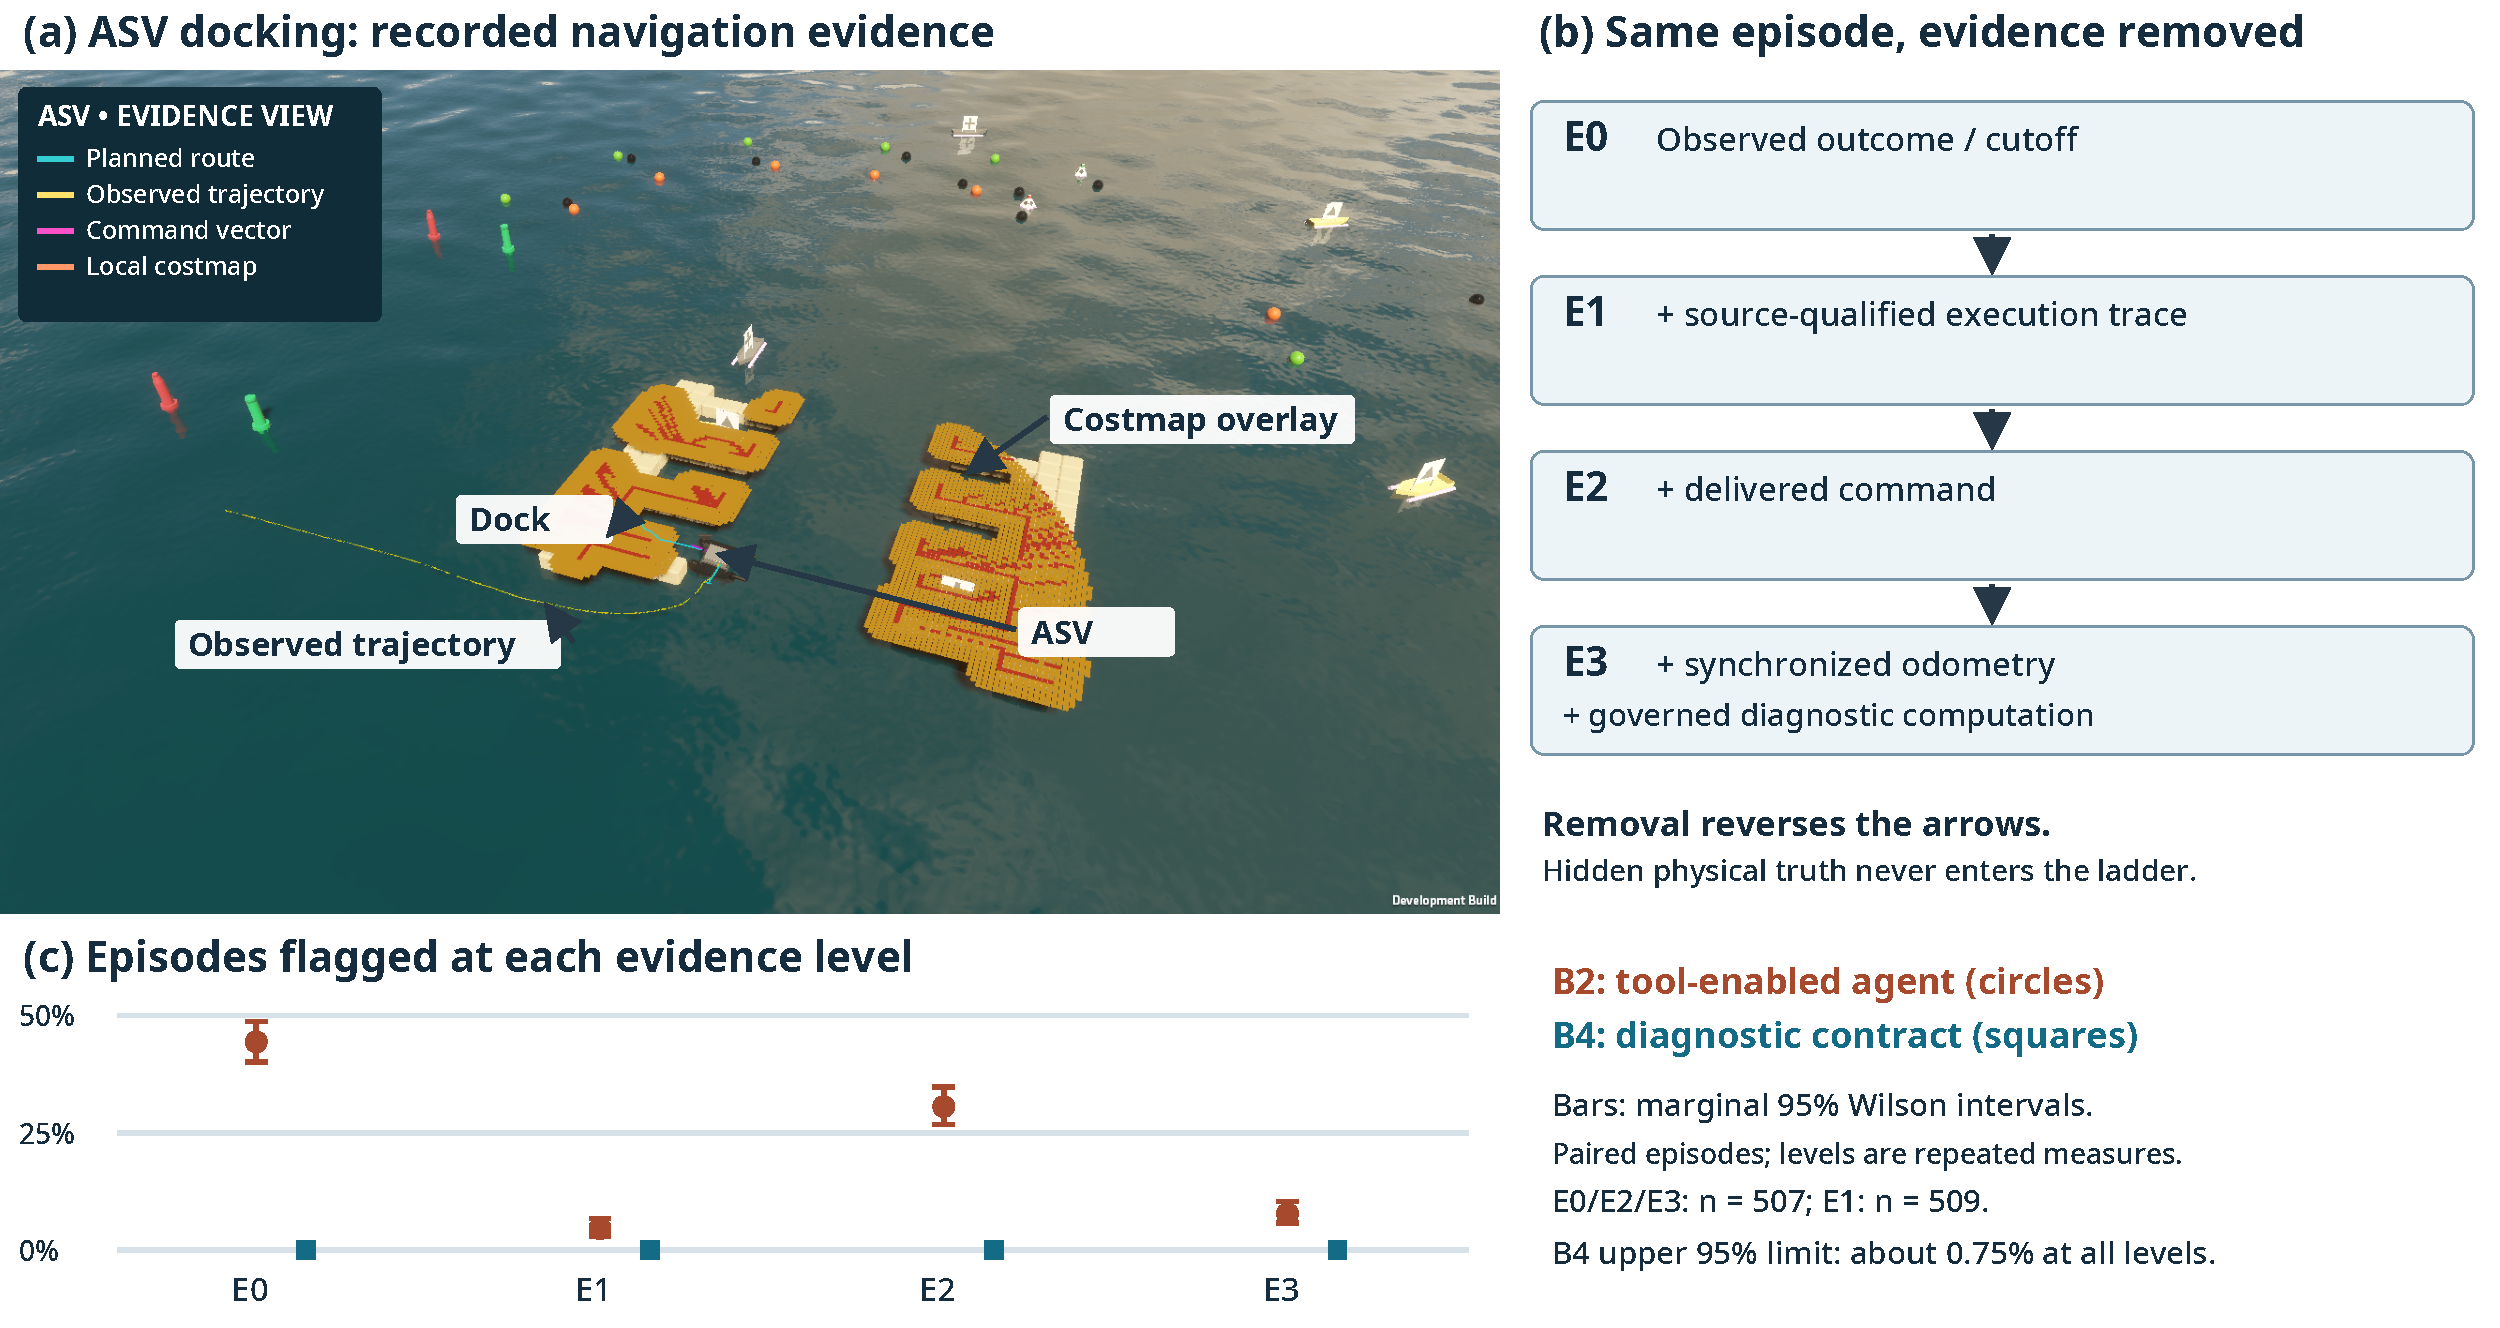
\includegraphics[width=\textwidth]{artifacts/extended-abstract-20261003/evidence-navigation-figure.pdf}
\caption{Evidence-grounded navigation explanations. \textbf{(a)} Simulated autonomous surface vessel (ASV) demonstration with dock, route, measured trajectory, command vector, and local costmap identified; this scene illustrates the evidence interface and is outside the quantitative land cohort. \textbf{(b)} The same physical land episode is presented under nested, removal-only evidence conditions. Delivered command plus synchronized measured motion can justify a discrepancy, but not a unique physical cause. \textbf{(c)} Exploratory automated rubric flags by evidence level: B2 has 225/507, 23/509, 155/507, and 39/507 adverse episodes; B4 has none. Bars show marginal Wilson 95\% intervals, not independent samples across levels.}
\label{fig:evidence}
\end{figure*}

\section{Three Contributions}
\textbf{C1: Evidence-calibrated explanation formalism.} Atomic claims have evidence requirements and diagnostic abstraction levels. Contracts preserve supported partial diagnosis, ambiguity, limitations, and rejection of false failure premises. Evaluator-only physical truth is separate from robot-visible support: \emph{physically true but unsupported} is an adverse category.

\textbf{C2: Controlled navigation benchmark.} Each physical episode is held fixed across removal-only masks: E0 provides outcome; E1 adds a source-qualified action/recovery trace; E2 adds delivered command; E3 adds synchronized odometry and governed diagnostic computation. The two analyzed families are persistent command--motion discrepancy and measured response recovery. Masks and claims remain clustered within episodes. E3 licenses a registered command--motion comparison; it does not identify motor failure, collision, slip, or a unique hidden cause.

\textbf{C3: Diagnostic-contract method and comparison.} B2 is a tool-enabled language-model agent with relevant evidence, source/configuration access, and local computation. B4 plans the maximal supported diagnosis, selects and orders permitted clauses, realizes exact numeric slots through templates, and verifies the result against the plan. This is constrained realization with explicit evidence checks.

\section{Evaluation and Retained Results}
A deterministic rubric extracts atomic claims from answer text, checks their evidence requirements against the visible level, and labels support, contradiction, insufficient evidence, physical truth without support, or uninterpretable content. It uses the same rules for both methods and does not read method identity or B4's internal clauses. An episode is flagged if any substantive claim on its available ladder is adverse. Parity checks, retained technical failures, removal-only masks, and deterministic reruns support traceability. The independent analysis unit is the episode, never the mask or claim.

The registered collection was administratively stopped before its first confirmatory look and before blinded annotation was dispatched. The present analysis was written after outputs were retained and is therefore exploratory automated scoring. We report the 511 episodes with at least one paired level and the 494 accounting-complete sensitivity; denominators differ by level (Fig.~\ref{fig:evidence}).

\begin{table}[t]
\centering
\caption{Exploratory retained-corpus results. Coverage is descriptive under the existing essential-unit inventory.}
\label{tab:results}
\footnotesize
\begin{tabular}{@{}lcc@{}}
\toprule
Measure & B2 agent & B4 contract \\
\midrule
Any adverse claim & 338/511 & 0/511 \\
\quad Wilson 95\% interval & 61.9--70.1\% & 0--0.75\% \\
Accounting-complete sensitivity & 325/494 & 0/494 \\
Unsupported causal-claim flag & 147/511 & 0/511 \\
Contradicted-claim flag & 43/511 & 0/511 \\
Essential-unit coverage at E3 & 0.897 & 0.952 \\
\bottomrule
\end{tabular}
\end{table}

The observed adverse-rate difference is $-66.1$ percentage points (B4 minus B2). B2's adverse labels include 420 insufficient-evidence claims, 45 contradiction flags, and four physical-truth-without-support labels. B4's communicated unit-category count rises from 1.76 at E0 to 4.76 at E3 under the operational rubric. Its coverage is lower at E0/E1 and higher at E2/E3: the result is a specificity--coverage tradeoff, with useful detail retained at the richest level, rather than evidence that shorter answers are inherently safer.

\section{Implications and Boundaries}
The study offers a reproducible way to ask \emph{which diagnostic claims become justified when evidence changes}. This addresses TNI-AIoT themes of reliable foundation-model agents, explainability and monitoring, dependable sensing-to-action processes, and reproducible benchmarks. Claim-level evidence checks provide a bounded reflection step over the execution record, helping researchers distinguish observations, diagnostic comparisons, and unresolved causes in natural-language reports. The ASV illustration separates software goal completion from sustained physical docking; no marine comparative result is claimed.

The current findings are simulation-only and rubric-relative. Template realization and scoring share an ontology, so B4's zero flagged rate is not proof of zero semantic error. Automated scoring is not human validation; coverage measures communicated contract units, not operator usefulness. One agent configuration cannot establish superiority over all agents. Independent semantic assessment, prospective replication, and operator evaluation remain necessary. The retained results motivate navigation explanations whose diagnostic detail follows their evidence.

\begin{thebibliography}{9}\footnotesize
\bibitem{reflect} Z.~Liu, A.~Bahety, and S.~Song, ``REFLECT: Summarizing robot experiences for failure explanation and correction,'' in \emph{Proc. CoRL}, PMLR 229, pp.~3468--3484, 2023.
\bibitem{hexar} T.~Love \emph{et al.}, ``HEXAR: A hierarchical explainability architecture for robots,'' arXiv:2601.03070, 2026.
\bibitem{ais} H.~Rashkin \emph{et al.}, ``Measuring attribution in natural language generation models,'' \emph{Comput. Linguist.}, vol.~49, no.~4, pp.~777--840, 2023.
\bibitem{factscore} S.~Min \emph{et al.}, ``FActScore: Fine-grained atomic evaluation of factual precision in long form text generation,'' in \emph{Proc. EMNLP}, pp.~12076--12100, 2023.
\end{thebibliography}
\end{document}
